Similar to the phase length analysis, we also vary the interval size, model, and similarity threshold and evaluate changes in phase transitions. As Figure~\ref{fig:phasetransavg} shows, as the interval size increases, the number of phase transitions tend to decrease. At higher thresholds, we see a separation in phase transition between IWS/BBV and ITD/CPI. Recall that in the phase length analysis, ITD tracked pretty closely with CPI as well and IWS and BBV tracked closely with each other. There appears to be a stabilization in the number of phase transitions at an interval size of 100 for the high threshold case for ITD and CPI, which coincides with the point at which the phase length for ITD and CPI begins to stabilize with increasing interval size as shown in Figure~\ref{fig:phaselen}. This suggests that increasing the interval size has the joint effect of increasing the phase length and decreasing the number of phase transitions, but that there does exist a stabilization point for which there will be little change in phase length and phase transitions. At low thresholds, we see very similar behavior in phase transition across models. In general, if a reconfiguration client is interested in lowering exploration costs by decreasing the number of phase transitions, it appears that the best avenue is to increase the interval size, but to also recognize there exists a limit as the number of phase transitions reaches it's minimum value and phase length reaches it's maximum value (i.e. a phase can not last longer then the duration of the program).  At higher thresholds, this stabilization in phase transitions and phase length occurs at a much earlier point as the interval size increases. 

\begin{figure}[htbp]
  \begin{center}
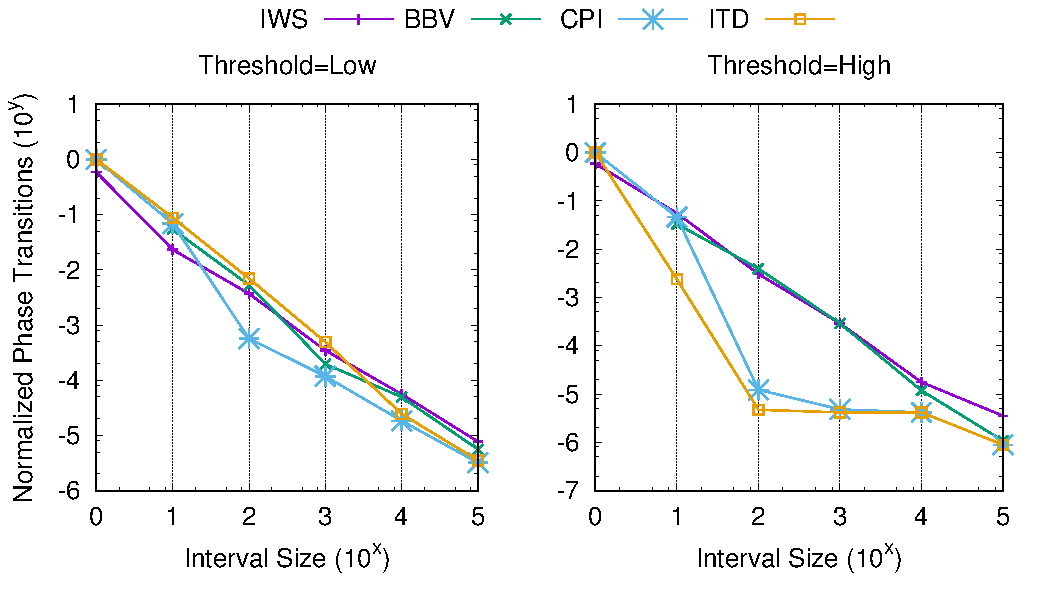
\includegraphics[width=0.95\columnwidth]{figs/phasetransavg}
  \end{center}
  \caption{The interval size is the most effective parameter for varying the phase transition compared with the model and threshold. But the threshold value does impact the rate at which the phase transitions decrease as the interval size grows and this behavior appears to vary between models.}
  \label{fig:phasetransavg}
\end{figure}


